\documentclass{beamer}
\DeclareFontShape{OT1}{cmss}{b}{n}{<->ssub * cmss/bx/n}{} 
\usetheme{default}
\usepackage{amsmath}
\usepackage{amsfonts}
\usepackage{mathbbol}
\usepackage{xcolor} % before tikz or tkz-euclide if necessary
\usepackage{tkz-euclide} % no need to load TikZ
\usepackage{multirow}
\usepackage{lmodern}
\usepackage{bm}

\title{Statistical Machine Learning\\ Part 6}
\author{Horacio G\'omez-Acevedo\\ Department of Biomedical Informatics}
\begin{document}
	\begin{frame}[plain]
		\maketitle
	\end{frame}
\begin{frame}
	\begin{figure}[h]
			\centering
			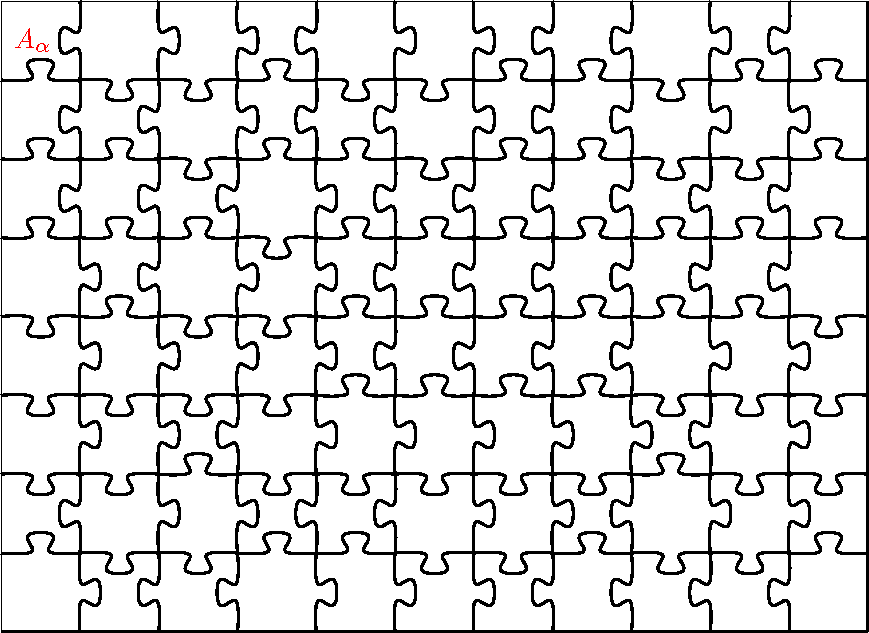
\includegraphics[scale=0.35]{../../Figures/fig_jigsaw.png}
		\end{figure}
\end{frame}

\begin{frame}{Resampling Methods for Parameter Estimation}
	Suppose you have applied your state of the art algorithm, but you don't know what is the distribution of a parameter (hyperparameter). The question is: how do I determine the bias and variance?
	
	The {\bf jackknife} and {\bf bootstrap} are {\it resampling} methodologies that help improving classification.
	
	
	 
\end{frame}

\begin{frame}{Jacknife}
	It was introducied by Maurice Quenouille around 1950's.  Let's start with an example as motivation for the use of the jacknife. 
	
	{\bf Example. } Let's suppose that we have 
	$m$ independent random variables $X_1,\ldots, X_m$ that follow the same distribution. We can define the statistic $\overline{X}$ defined as $\frac{X_1 + \cdots + X_m}{m}$. The question is what is the standard deviation of this statistic given a set of observed values $X_1=x_1,\ldots, X_m=x_m$?
	
	Following the definition of variance, we can determine
	
	\begin{equation}
		\widehat{\sigma}^2(\overline{X})= \frac{1}{m(m-1)} \sum_{i=1}^m (x_i - \overline{x})^2
		\label{eq:stdev}
	\end{equation}
	
	That was simple enough, but what about calculating an estimate of the variance for other common statistics as  {\it mode}, or {\it median} or other statistics?
	
\end{frame}

\begin{frame}{Jackknife}
	Let's define the sample average of the data set deleting the jth variable as
	\begin{equation*}
		\overline{X}_{(j)}= \frac{1}{m-1} \sum_{k\ne j} X_k
	\end{equation*}
We also define the statistic that is the {\it average} of these averages
\begin{equation*}
	\overline{X}_{(\bullet)} = \frac{1}{m} \sum_{k=1}^m \overline{X}_{(k)}
\end{equation*}

The {\bf Jackknife} estimate of the standard deviation is
\begin{equation}
	\widehat{\sigma}_{Jack}^2(\overline{X})= \frac{m-1}{m} \sum_{i=1}^m (\overline{X}_{(i)} - \overline{X}_{(\bullet)})^2
\label{eq:jstdev}
\end{equation}

It can be verified that (\ref{eq:stdev}) and (\ref{eq:jstdev})  coincide; however, this process allows a generalization of this method.
\end{frame}

\begin{frame}{Jackknife}
	One of the biggest advantages of the expression (\ref{eq:jstdev}) is that when we  have an estimator $\hat{\theta}(x_1,\ldots, x_m)$ of the statistic $\theta$, we can actually estimate the variance of such estimator
	\begin{equation*}
		\hat{\sigma}_{jack}^2= \frac{m-1}{m} \sum_{i=1}^m (\hat{\theta}_{(i)}- \hat{\theta}_{(\bullet)})^2,
	\end{equation*}
where
\begin{equation*}
	\begin{split}
		\hat{\theta}_{(i)}&= \hat{\theta}(x_1, \ldots, x_{i-1},x_{i+1},\ldots, x_m) \\
		\hat{\theta}_{(\bullet)}&= \frac{1}{m-1} \sum_{i=1}^n \hat{\theta}_{(i)} 
	\end{split}
\end{equation*}

\end{frame}
		
\begin{frame}{Jackknife bias}
	It is also possible to obtain the {\bf jackknife bias} estimation
	
	Recall the definition of bias
	\begin{equation*}
		bias = \theta - E(\hat{\theta})
	\end{equation*} 
The Jackknife estimate of bias is given by

\begin{equation*}
	bias_{jack}= (m-1) (\hat{\theta}_{(\bullet)}- \hat{\theta})
\end{equation*}
\end{frame}		
		
\begin{frame}{Bootstrap}
	In a common definition, a {\it bootstrap} data set is one created by randomly selecting $m$ points (with replacement) from the training set $\cal{D}$.
	
	For example if our training data set consists of the points $\{(x_1,y_1),(x_2,y_2),(x_3,y_3)\}$, then a bootstrap could be 
	
	\begin{equation*}
		\begin{split}
				B_1&=\{(x_1,y_1),(x_2,y_2),(x_3,y_3)\}\\
				B_2&=\{(x_1,y_1),(x_1,y_1),(x_2,y_2)\} \\
				B_3&=\{(x_2,y_2),(x_3,y_3),(x_2,y_2)\} 
		\end{split}
	\end{equation*}
	 
\end{frame}		

\begin{frame}{Bootstrap}
	In the bootstrap setup, the data sets (say $B_j$s in our example) are treated as independent sets. The {\bf bootstrap} estimate of a statistic $\theta$ is defined as
	
	\begin{equation*}
		\hat{\theta}^{*(\bullet)}= \frac{1}{B} \sum_{b=1}^B \hat{\theta}^{*(b)},
	\end{equation*}
where $\hat{\theta}^{*(b)}$ is the estimate of $\theta$ for the sample $b$ .
\end{frame}		

\begin{frame}{Bootstrap bias and variance estimates}
	The bootstrap estimate of the bias 
	\begin{equation*}
		bias_{boot}= \hat{\theta}^{*(\bullet)}- \hat{\theta}
	\end{equation*}
	Whereas the bootstrap estimate of the variance is
	\begin{equation*}
		\hat{\sigma}^2 (\theta)= \frac{1}{B}\sum_{b=1}^B \left(  \hat{\theta}^{*(b)} - \hat{\theta}^{*(\bullet)} 
		\right)
	\end{equation*}
\end{frame}
		
	\begin{frame}{References}
		
		Materials and some of the pictures are from (1),(2), and (3).
		\begin{enumerate}
			\item Gareth James et al. {\it An Introduction to Statistical Learning with applications in R}. Springer (2015)
			\item Richard O. Duda et al. {\it Pattern Classification} John Wiley (2001). 
			\item Aur\'elien G\'eron. {\it Hands-on Machine Learning with Scikit-Learn \& TensorFlow} O'Relly (2017)
			\item Wiebe R. Pestman {\it Mathematical Statistics} de Gruyter (1998)
			\item Bradley Efron. {\it The Jackknife, the Bootstrap and other Resampling Plans}  SIAM (1982)
		\end{enumerate}	
		
		I have used some of the graphs by hacking TiKz code from StakExchange, Inkscape for more aesthetic plots and other old tricks of \TeX
	\end{frame}	

	
\end{document}